% !Mode:: "TeX:UTF-8" (encoding info for WinEdt)
\section{Visualisation des images dans Elexis}
Intégration des photos et d'autres images dans le texte de consultation. Ce Plugin fait partie de la distribution standard. Pour intégrer une image externe vous procédez de façon suivante :
Veuillez bouger la flèche sur l'endroit où vous voulez intégrer l'image et cliquez droit.

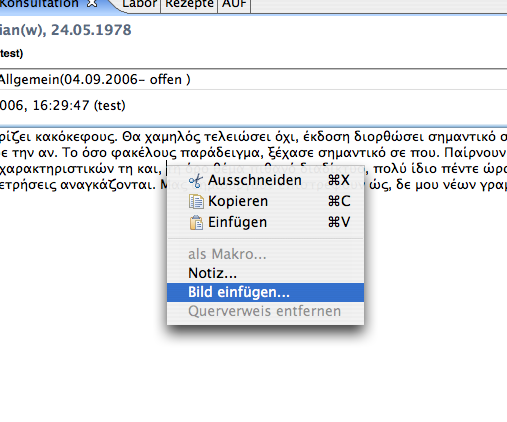
\includegraphics[width=4in]{images/bild1}
% bild1.png: 507x422 pixel, 72dpi, 17.89x14.89 cm, bb=0 0 507 422


Cliquez \textit{intégrer image...} et choisissez dans la fenêtre qui s'ouvre l'image souhaitée. (Les images doivent être des formats JPG, GIF ou PNG). L'image sera importée dans la base de données et une référence sera introduite dans le texte.(L'image originale ne sera plus utile et pourrait être effacée.)

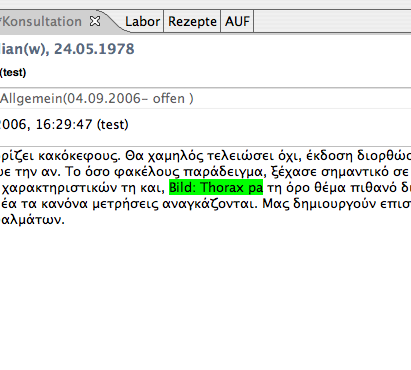
\includegraphics[width=3in]{images/bild2}
% bild2.png: 411x370 pixel, 72dpi, 14.50x13.05 cm, bb=0 0 411 370


En cliquant sur le lien on peut laisser afficher l'image à tout moment.

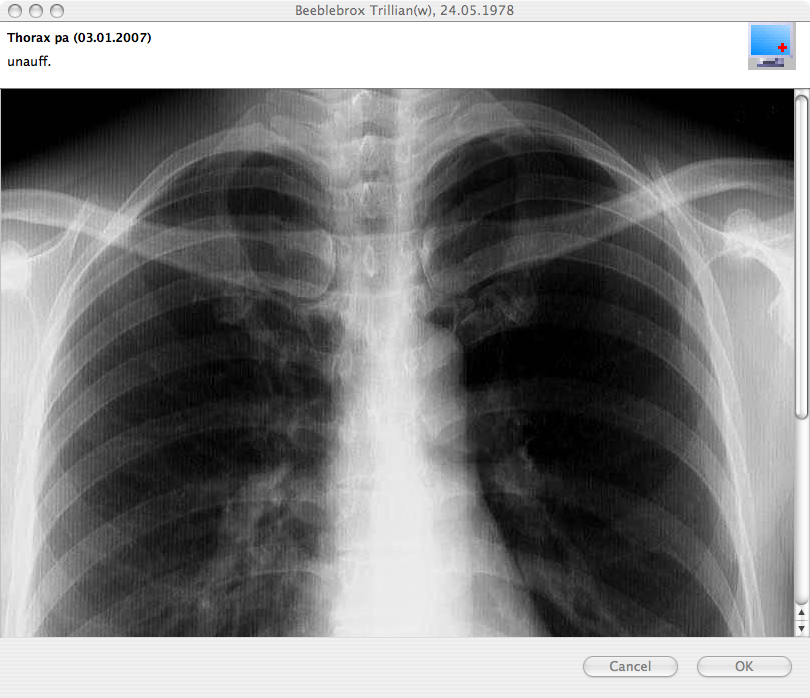
\includegraphics[width=4in]{images/bild3}
% bild3.png: 810x698 pixel, 72dpi, 28.58x24.62 cm, bb=0 0 810 698
